\documentclass[border=2pt]{standalone}
\usepackage{tikz}
\usepackage{amsmath}
\usepackage{mathtools}
\usepackage{adjustbox}
\usetikzlibrary{patterns}
\usetikzlibrary{calc} \usetikzlibrary{positioning} \usetikzlibrary{shapes,arrows} \usetikzlibrary{plotmarks}
\usetikzlibrary{positioning,decorations.pathreplacing}
\tikzset{
litria/.style={
  draw,shape border uses incircle,
  isosceles triangle,shape border rotate=90,yshift=-0.3cm,xshift=0.1cm},
ritria/.style={
  draw,shape border uses incircle,
  isosceles triangle,shape border rotate=90,yshift=-0.3cm,xshift=-0.1cm}
}

\begin{document}

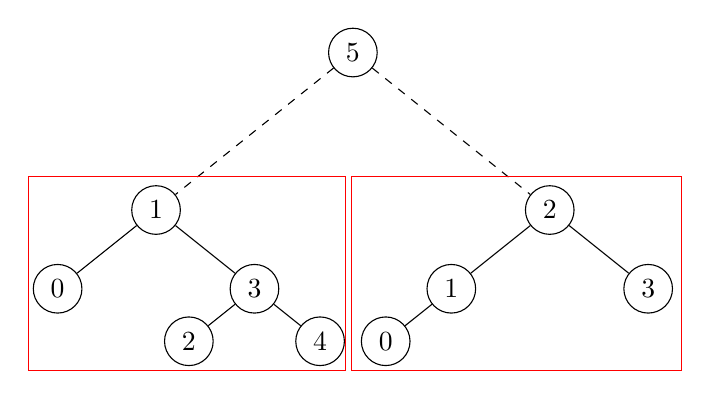
\begin{tikzpicture}[level/.style={sibling distance=50mm/#1, level distance=20mm/#1},baseline=(root.base)]
\node[circle,draw](root){$5$}
    child[dashed] { node[circle,draw,solid](lson){$1$}
        child[solid] { node[circle,draw]{$0$}
        }
        child[solid] { node[circle,draw]{$3$}
          child { node[circle,draw]{$2$}
          }
          child { node[circle,draw](lson-rightmost){$4$}
          }
        }
    }
    child[dashed] { node[circle,draw,solid](rson){$2$}
        child[solid] { node[circle,draw]{$1$}
          child { node[circle,draw]{$0$} }
          child[missing]{}
        }
        child[solid] { node[circle,draw](rson-rightmost){$3$}
        }
    }
  ;

\coordinate (lsonLL) at ([yshift=0.2cm,xshift=-1.4cm] lson.north west);
\coordinate (lsonRR) at ([yshift=-0.15cm,xshift=.1cm] lson-rightmost.south east);

\coordinate (rsonLL) at ([yshift=0.2cm,xshift=-2.3cm] rson.north west);
\coordinate (rsonRR) at ([yshift=-0.81cm,xshift=.2cm] rson-rightmost.south east);

\draw[red] (lsonLL) rectangle (lsonRR); 
\draw[red] (rsonLL) rectangle (rsonRR); 

\end{tikzpicture}

\end{document}